\chapter{Etats de l'art}
\label{ch:state_art}

\section{introduction}
Dans ce chapitre, nous aborderons les différentes pistes envisagées afin de remplir les objectifs fixés dans cette thèse, comme listés dans l'introduction (\cf{ch:introduction}).

Avant toutes choses, il a fallu se mettre au niveau et comprendre la thèse \thLeite.

\section{Automatisation}
En terme d'automatisation, une pratique bien courante chez les développeurs s'agis d'utiliser des scripts bash afin de pouvoir exécuter un certain nombre de commande et de code successivement. Bien que cette méthode présente l'avantage d'êtres simple, il suffit d'une console UNIX et d'un éditeur de texte, elle présente un défaut majeur. En effet, le développeur du script contrôle quel commande et code sont exécutés et peut également définir des paramètres pour ceux-ci, mais il ne peut pas contrôlé l'environnement d'exécution.

Une façon de faire, en plein essor depuis quelque temps, est l'utilisation de la plateforme Docker. Il s'agit d'un logiciel de containerisation. C'est-à-dire la création de brique d'application, qui mise en communes permet de réaliser une application globale. De plus, le développement d'une telle solution permet un partage facilité grâce à un déploiement facilité et autonome. Pour davantage d'explication sur le sujet je vous renvoie au chapitre  \cf{ch:docker}.

Vous l'aurez bien compris, le choix qui a été fait est celui de l'utilisation de Docker.

\section{Configuration}

En ce qui concerne la recherche d'une méthode afin de réaliser facilement des fichiers de configurations précréées, beaucoup de solutions existent. Ces différentes méthodes sont plus ou moins flexibles aux modifications.

Les fichiers de configurations dont il est question ici sont spécifiques à la partie python du code qui sera exécuté par notre application \cf{ch:app}. En effet, l'on souhaite entre autres être capable de donner des fichiers de configuration en entrée et d'obtenir pour chacun un résultat en sortie.

Nous citerons ici uniquement la solution retenue, car les autres solutions trouvées sont soit trop incompatibles soit presque identiques à la solution retenue.

Nous utilisons le module python \emph{Configparser}, qui permet de lire et parser des fichiers à l'extension .ini de manière simple. De plus, la structure d'un fichier .ini est très simple et ne laisse donc que très peu de place aux erreurs de format.
 
 
\section{Hmmer}
Dans la thèse \thLeite les séquences protéiniques sont recherchées dans la base de données de profile-HMM à l'aide d'une \gls{api} en ligne. Cette \gls{api} est disponible depuis le site \emph{https://www.ebi.ac.uk/Tools/hmmer/}. 

Comme dis précédemment, un des objectifs de ce travail est de se passer de l'utilisation de cette \gls{api} car sont accès n'est pas toujours disponible ou stable.

Une recherche rapide à permis de se rendre compte que l'application utilisée derrière cette \gls{api} est disponible au téléchargement et peut donc êtres utilisée de manière locale. Pour davantage d'information \cf{ch:app}, sous-chapitre Hmmer.


\section{Parallélisation}

La version existante du code se trouvant dans la thèse \thLeite est une version sous forme de script, proof-of-concept, en python2 et non \emph{multiprocessed}. Afin de garantir une utilisation optimale des ressources de la machine hôte, sur laquelle le code est exécuté, nous souhaitons rendre le code parallèle là où il est possible de le faire.

Plusieurs solution sont possible, encore une fois les solutions les plus compliquées ne sont pas toujours celle les plus efficaces. De plus une méthode trop complexe pourrait réduire la bonne transmission du code à d'autres développeurs.

La partie principale que l'on souhaite paralléliser est l'utilisation de la fonction de scanne de HMMMER, étant donné qu'un très grand nombre de séquences protéiniques doivent être analysées.

\subsection{Simple}
\subsubsection{Docker}
Docker, mis à part de rendre le déploiement et l'exécution d'application automatisée, permets également de lancer plusieurs conteneurs simultanément, \cf{ch:docker}. Un conteneur englobe un système de fichier complet possédant tous se qu'y est nécessaire a remplir sa fonction. 

\subsubsection{Python}
En python on retrouve deux principales méthodes permettant de réaliser de code parallèle. En effet, on peut utiliser le \emph{multiprocessing} ou le \emph{multithreading}.

Notre bute est de réaliser et d'optimiser un code \gls{cpu} dépendant, c'est-à-dire coeurs dépendants. Lors de l'utilisation du langage python il faut savoir qu'avec des codes \gls{cpu} dépendants, python limite les possibilités de parallélisme à cause de la \gls{gli}. La \gls{gli} est nécessaire en python, car python n'est pas \emph{tread safe}. En effet, il y a, en python, un verrou global lorsque l'on essaye d'accéder à un objet depuis un thread.

À cause de se verrous les codes \gls{cpu} dépendants ne gagneront pas en performance lorsqu'ils sont parallélisés à l'aide de \emph{multithreading}, mais uniquement avec le \emph{multiprocessing}.

\subsection{Avancée}
\subsubsection{Docker Swarm}
Une autre méthode utilisant une librairie avancée de Docker, consiste à utiliser Docker Swarm. Docker Swarm apporte à Docker une gestion native du \emph{clustering}, afin de transformer un groupe de \emph{Docker engines} en un unique et virtuel \emph{Docker engine}. Grâce à cela, il est possible d'exécuter une application sur une architecture partagée sur plusieurs systèmes physiquement indépendants. 

\subsubsection{Spark}
Spark est un framework \emph{open source} de calcul distribué. Il permet d'effectuer des analyses complexes sur un grand nombre de données.

Il est également un ensemble d'outils pour le traitement de grande source de données, notamment grâce à des fonctions \emph{MapReduce}.
	
\section{Optimisations}
Le code repris de la thèse \thLeite est un code séquentiel, sous forme de script nécessitant des inputs utilisateurs a chaque étape. De plus, ce code est ecrit en python dans sa version 2.

Grâce au travail du Dr. Brett Cannon, \href{https://speakerdeck.com/pyconslides/python-3-dot-3-trust-me-its-better-than-python-2-dot-7-by-dr-brett-cannon}{voir ici}, on se rend compte que python 3.3 pourrait optimiser les performances de notre application. On peut lire  \href{https://mail.python.org/pipermail/python-dev/2012-October/121923.html}{ici} que même l'appel des fonctions est en moyenne 1.20 fois plus rapide. De plus, les \emph{threadded count} sont également plus rapide.

Une autre possibilité est d'utiliser \emph{Cython}. Cython est un compilateur/langage de python permettant d'utiliser des appeles au langage C et de compiler un code python en exécutable C. Il faut savoir qu'un exécutable C est généralement plus rapide que l'exécution de l'interpréteur Python. 

On trouve le tableau suivant dans la documentation de Cython, qui permet de nous rendre compte des différences.

\begin{figure}[H] 
\centering 
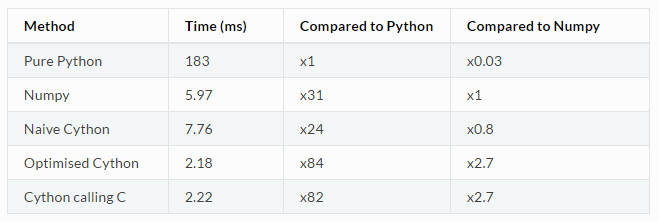
\includegraphics[width=1\columnwidth]{img/table_cython} 
\caption[Tableau performences Cython]{Tableau de comparaison de Cython - \url{http://notes-on-cython.readthedocs.io/en/latest/std_dev.html/}).}
\label{fig:galleria} 
\end{figure}

\section{conclusion}
Après des tests sur ces différentes technologies et méthodes et quelques discutions ici et là, l'idée ayant été arrêté est d'utiliser \emph{Docker} et \emph{Docker Compose} comme contexte applicatif et de transformer les scripts en une application orientée objet en python 3.3 gérant les fichiers de configurations avec la librairie \emph{Configparser}. Pour ce qui est du parallélisme, il sera réalisé en utilisant la librairie \emph{Multiprocess}.
















